%% ----------------------------------------------------------------
%% Experiment.tex
%% ---------------------------------------------------------------- 
\chapter{RetinaNet Deployment} \label{Chapter:Experiment}
This chapter covers an analytical, detailed review upon the system deployment, the proposed architectures and the hyper-parameter selection accompanied with the respective reasoning behind every choice. It also presents how performance scales in function with the dataset training size. Later proceeds to overall tuning with the most appropriate hyper-parameter values to obtained peak detection and counting.

\section{Dataset Description}
The authors of the papers \cite{bargoti2017image} and \cite{bargoti2017deep} introduced the dataset used in this study and is provided through the Australian Centre or Field Robotics (ACFR), The University of Sydney\footnote{\url{http://data.acfr.usyd.edu.au/ag/treecrops/2016-multifruit/}}. The images were collected using the platform "Shrimp", an unmanned ground vehicle in apple, mango and almond orchards. However, in this study, only the apple subset was used.

Precisely, the dataset consists of random crops from images that span entire trees, trellised in the orchard block. The total number of apple instances in the images represents the total number of fruits in the orchard block. The split in training, validation and test set follows the proposed split from authors' previous work, to provide valid comparisons with the previous literature work. \tref{tab1} summarises an overview of the dataset.

\begin{table}[!htb]
  \centering
  \resizebox{\textwidth}{!}{
  \begin{tabular}{cccccc}
  \toprule
  \textbf{Set} & \textbf{Raw Img. Size} & \textbf{Cropped Img. Size} & \textbf{No. of Img.} & \textbf{Fruit Width} & \textbf{Fruits/Img.} \\
  \midrule
  train 		& $1616\times1232$ & $202\times308$ & 896	& $36.27 \pm 7.55$  & $5.22 \pm 3.37$\\
  val. 		& $1616\times1232$ & $202\times308$ & 112 	& $35.92 \pm 7.83$  & $4.80 \pm 3.10$\\
  test. 		& $1616\times1232$ & $202\times308$ & 112 	& $35.29 \pm 7.30$  & $4.95 \pm 3.21$\\
  train + val. 	& $1616\times1232$ & $202\times308$ & 1008	& $36.23 \pm 7.58$	& $5.17 \pm 3.35$\\
  \bottomrule
  \end{tabular}
  }
  \caption{ACFR dataset description}
  \label{tab1}
\end{table}

The dataset provides circular annotations for the fruits; thus, they were converted to squares with the same width and height. Instead of discarding annotations that exceed the borders of the image, they were clipped to fit the image.
 
\section{Proposed Deployment and Configuration}
\subsection{Hardware and Software specifications}
The deployment was set up on the Keras (\cite{chollet2015keras}) implementation of RetinaNet, provided by Fizyr\footnote{\url{https://github.com/fizyr/keras-retinanet}} and trained using a single NVIDIA Ge Force GTX 1080 Ti provided by the Iridis 5\footnote{\url{https://www.southampton.ac.uk/isolutions/staff/iridis.page}} Computer Cluster. Appendix \ref{pack_versions} includes the complete list with the packages' versions. The repository can be found in \url{https://github.com/nikostsagk/Apple-detection}.

\subsection{Training Details}
The models were trained for 30 epochs of 2000 steps each with $\text{batch size} = 1$. Regarding the optimiser, ADAM (\cite{kingma2014adam}) was used, with an initial learning rate of $10^{-5}$, decreased later by a factor of 10 on epoch 15 and again on 25. It was observed that the models did not show any signs of overfitting as the performance on the validation set was increasing until it stabilised around its maximum value; meanwhile, the validation loss was fluctuating around a minimum value. All models were initialised on the ImageNet VGG16 pre-trained weights unless otherwise stated. 30 epochs of training time took around 80-90 minutes for each model, but the performance had reached its peak from the first 5 epochs.

All models were trained on the training set monitoring performance on the validation set. Performance metrics stated here, refer to performance on the test set unless otherwise indicated.

\subsection{Data Augmentation \& Preprocessing}
Originally, RetinaNet was trained on images with a minimum side of 800. Therefore, first tries adopted this strategy, keeping the ratio unchanged (e.g. $800\times1220)$. Later, to save upon training and inference time, a resolution of $512\times781$ was proposed ensuring that at least one pixel can represent a fruit in the last layer (P7). Finally, the resolution utilised in all models was the original $202\times308$ as no model showed any gain in performance with higher resolutions. By adopting the original resolution, there are considerable earnings in training and inference time giving the opportunity to train multiple models.

The data augmentation techniques used were along with the natural variations of the dataset. Specifically, the augmentations included random flipping along the x-axis with 0.5 chance and random photometric transformations such as \textit{Fancy PCA} (as described in \cite{taylor2017improving}), changes in brightness/contrast, and finally changes in the HSV colour space. Instead of expanding the dataset before training begins, each sample is randomly undergoing a random augmentation during training, avoiding pre-calculations. Besides the augmentation, the ImageNet mean values were subtracted from the dataset as the VGG16 was initially trained that way.

\subsection{Anchor Boxes Configuration}
Instead of using the default anchor boxes' base size, ratios and scales, a common practice used in anchor-based detection pipelines (\cite{redmon2017yolo9000}, \cite{redmon2018yolov3}) is to use k-means clustering, over the dataset where the $k$ centroids' width and height define anchors' base size. Nonetheless, this practice cannot be adopted in this dataset, as the variance among the size of the fruits is small enough, and all centroids would have similar dimensions.

However, the anchor configurations are optimised through a differential evolution search algorithm (\cite{storn1997differential}) as in \cite{zlocha2019improving}. The algorithm starts with the default anchor boxes' configuration: $\text{base size} = (32^2, 64^2, 128^2, 256^2, 512^2)$, $\text{ratios} = (1\!:\!2, 1\!:\!1, 2\!:\!1)$ and $\text{scales} = (2^{0}, 2^{1/3}, 2^{2/3})$ and through candidate populations try to minimise the distance = $1 - IoU_{avg.}$, that is to maximise the average overlap between anchors and ground truth boxes. For computational efficiency, the algorithm considers only reciprocal ratios = $(1/x, 1, x/1)$ on the validation dataset. \tref{tab2} summarises the proposed anchor configuration. \\

\begin{table}[!htb]
  \centering
  \begin{tabular}{cc}
  \toprule
  \multicolumn{2}{c}{\textbf{Anchor Settings}} \\
  \midrule
base size	& 	\small{$(32^2, 64^2, 128^2, 256^2, 512^2)$} \\
stride 	& 	$(8, \ 16, \ 32, \ 64, \ 128)$ \\
ratios  	&	$(0.805, \ \ 1.0, \ \ 1.242)$ \\
scales  	& 	$(0.696, \ \ 1.0, \ \ 1.313)$ \\
  \bottomrule
  \end{tabular}
  \caption{The suggested anchor boxes' configuration proposed by the differential evolution search algorithm. The average IoU between anchor boxes and ground truth, is 0.994.}
  \label{tab2}
\end{table}

 \fref{fig1} illustrates how anchor boxes' area spans the distribution of on the training and validation annotations' area. It is evident that the anchors coming only from the two first layers are enough and span the dataset adequately. A reasonable question would be why the anchor box base size is not reduced even further to span the entire dataset more densely? The reason is that deeper layers, have larger receptive fields and are responsible for the detection of bigger objects; furthermore, the stride increases rapidly in deeper pyramid layers thus smaller anchors would not be able to span the entire feature map densely. This observation justifies the curiosity in exploring shallower alternatives of the original model.
 
\begin{figure}[!htb]
  \centering
  \subfigure[Training dataset.]{
    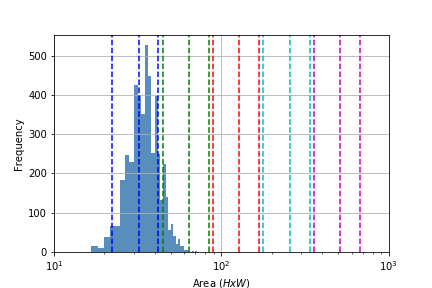
\includegraphics[width=0.45\textwidth]{figures/ch3/fig1_1.png}
    \label{fig1_1}
  }
  \subfigure[Validation dataset.]{
    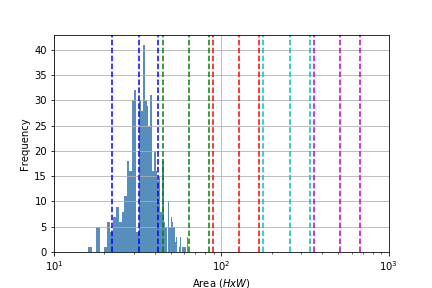
\includegraphics[width=0.45\textwidth]{figures/ch3/fig1_2.png}
    \label{fig1_2}
  }
  \caption{The annotation boxes' area distribution, along with the scaled optimised anchor boxes. It can be seen that the anchors coming from the last 3 layers are almost redundant.}
  \label{fig1}
\end{figure}

\subsection{Hyper-parameter Selection}
The IoU threshold to consider a detection as a true positive was set equal to $IoU_{th} = 0.2$ (as in \cite{bargoti2017deep} to perform valid comparisons), unless otherwise stated. The confidence score for the proposed detections was set as $p(c_i) > 0.05$ and the $\text{NMS}_{th}$ was set equal to 0.3 as it found out to be the best after experimentation. To save computation time, the maximum proposed detections allowed was set to be 100. 

Lastly, concerning the loss function, tweaking $\alpha$ and $\gamma$ did not yield any difference in performance, so the default parameters $\alpha=0.25$ and $\gamma=2$ were adopted. A notable remark is that the loss function found to be very unstable during training, and the reason was the normalisation parameters, which they take values equal to traintr'''the total number of instances in the image. This behaviour was a result of the Fruit/Img. deviation as it can be found in \tref{tab1} very large. To tackle this issue, the normalisation factor was modified, taking values from an exponential moving average of the total instances in the samples.
 
\subsection{Proposed Architectures}

\section{VGG Architectures Comparisons}

\section{Performance - Training Size Relation}

\section{Peak Detection and Evaluation}

\dots